%%%%%%%%%%%%%%%%%%%%%%%%%%%%%%%%%%%%%%%%%%%%%%%%%%%%%%%%%%%%%%%%%%%%%%%%%%%%%%%%
%neutrino_physics.tex: Chapter on neutrino physics:
%%%%%%%%%%%%%%%%%%%%%%%%%%%%%%%%%%%%%%%%%%%%%%%%%%%%%%%%%%%%%%%%%%%%%%%%%%%%%%%%
\chapter{Physics of Neutrinos}
\label{neutrino_physics_chapter}
%%%%%%%%%%%%%%%%%%%%%%%%%%%%%%%%%%%%%%%%%%%%%%%%%%%%%%%%%%%%%%%%%%%%%%%%%%%%%%%%

\section{Standard Theory in a nutshell}
\begin{figure}
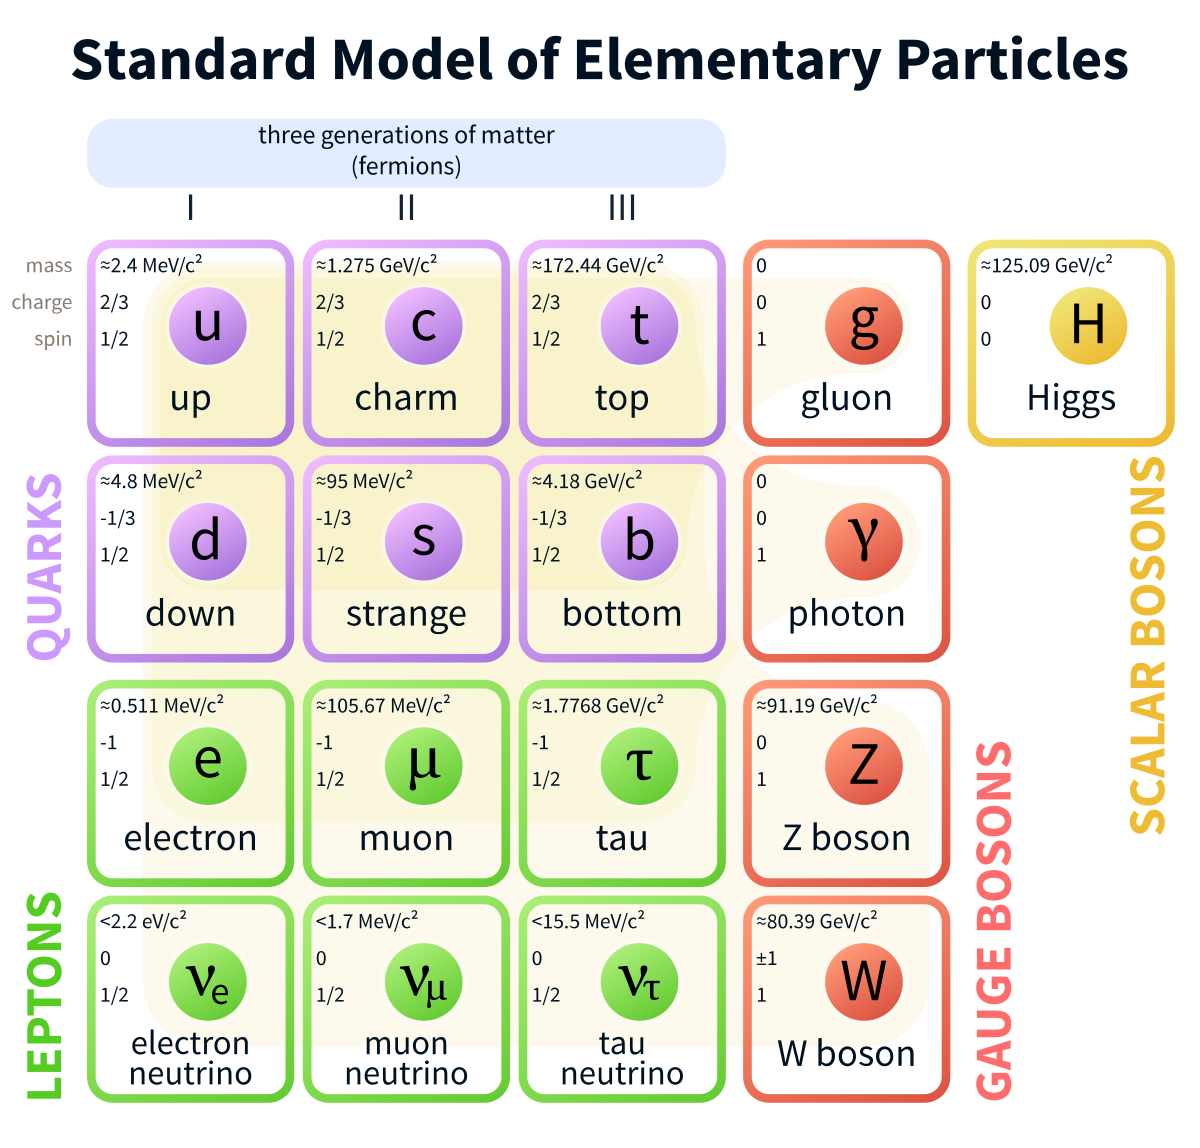
\includegraphics[width=0.8\textwidth]{figures/Standard_Model_of_Elementary_Particles.png}
\centering
\caption{Elementary Particles in the Standard Theory.} \lb{SM}
All particles could be divided into 2 groups: fermions and bosons. Fermions are 
further divided into quarks with fractional charges and leptons - charged ones ($e, \mu, \tau$)
and neutral ($\nu_e, \nu_\mu, \nu_{\tau}$). The fermions participate in strong (except leptons), 
weak and (only charged ones) electromagnetic interactions. These interactions are 
mediated by massless gluons ($g$), massive weak bosons $W^{\pm}$ and $Z^0$ and massless
photon ($\gamma$). The Higgs boson is last discovered particle and is reponsible all others 
particles' masses.
\end{figure}
Since ancient times people were trying to understand the world around them. From 
first world models of ancient Greeks to modern theories scientists tried to use 
limited number of entities to decribe phenomena happened in nature - Democritus's 
indivisible atoms, Plato's elements (air, fire, water, earth) or elementary particles 
of the Standard Theory. Here we focus on the latest and most accurate theory - the
Standard Theory.

Elementary particles of the Standrar Theory are the building blocks of matter, and the glue of everything we
can see around us\footnote{As of today, Standard Theory and Einstein's General Theory of 
Relativity could not fully explain motion of galaxies and exponential expansion of the Universe. 
Two more entities were introduced - dark matter for former phenomenon and dark energy 
for latter one.}. However, the most fascinating thing about the Theory is that underlying 
principles that governs it are symmetries - gauge symmetry and Lorentz 
symmetry. The Standard Theory's group is 
\be
SU(3)\times SU(2)\times U(1),
\ee 
where the $SU(3)$ group describes strong interactions, and the $SU(2)\times U(1)$ group describes 
electro-weak interactions\footnote{Gravitational interaction falls out of the picture
since for the last one hundred years gravity is described by deformation of space-time 
continium. Nevertheless, the attempts to rewrite gravity using the same language of groups
and unified it with Standard Model never were given up. In fact, all latest unified theories 
were based on groups of high demenstions where one of the most promising theories is 
String Theory.}. The different mathematical properties of the groups naturally split
the particles into two categories based on their spins: bosons and fermions. Fermions are 
particles with half-integer spin and bosons are particles with integer spin (in units of $\hbar$). 
The matter consists of fermions, while bosons serve for carrying interactions between matter particles.

Fermions in the Standard Theory are quarks and leptons. Quarks make up protons
and neutrons and have fractional electric charge - up, charm and top quarks have charge $+\frac{2}{3}e$, 
while down, strange and bottom have $-\frac{1}{3}e$. Quarks also have strong charge - color -
which could be one of three options: green, red or blue. The interesting fact is that the quarks
are not observable in the same sense as electrons could be observable and only three (baryon) or 
two-quark (meson) combinations exist\footnote{Recently, five quark combinations have been discover}. 
This phenomenon is called quark confinement with no complete explanation as of today. 

The other sector of the Standard Theory - the lepton sector - cosnists of negatively charged electron,
muon and tau particles as well as neutral neutrinos. These particles participate only in
weak and electromagnetic interactions. Moreover, the electron and electron neutrino carry an electron 
lepton number, similar quantities are carried by muon and tau leptons. Lepton numbers are known to be 
conserved in every process, for example, muon decay produces not only electron but corresponding muon 
neutrino and electron antineutrino. Although attempts to observe lepton number violation are being made.

As shown in figure \p{SM}, fermions are split into three generations. The mass of each 
subsequent generation is bigger by at least two orders of magnitude. The matter we observe 
around us is made of particles from first generation. Why do other generations exist? Why are
there only three generations? Physicists do not know the answer to this questions, nor 
why there is a gigantic ($10^{11}$) mass difference between the lightest and the heaviest particles. 

The last but not the least sector of the Standard Theory is boson sector. This sector is 
represented by particles which mediate electromagnetic, weak and strong interactions. The photon
($\gamma$) is spin-1 massless carrier of the electromagnetic force and is reponsible for almost all phenomena 
that a person experiences in their life - from the Sun's light, to the frictions and atomic bonds between 
chemical elements. Only charged particles interact through photon exchange.

The strong force carrier is spin-1 massless gluon ($g$). Gluon exchange binds quarks into stabel states asi
baryons - protons, neutron etc - or mesons - $\pi$, $\rho$ etc. While the photon is electrically
neutral and can not interact directly with other photons, gluon carries a color or
rather color-anticolor and can interact with other gluons. As mentioned earlier, only specific 
combinations of quarks are observable - colorless combinations - three quarks of different colors,
or quark-antiquark pairs with color-anticolor charge. In strong interaction quark changes its color
by emitting gluon, for example, a blue quark emits blue-antired gluon and becomes a red quark.

The weak force carriers are spin-1 massive $W^\pm$ and $Z^0$ bosons. All the Standard Theory fermions 
can interact via weak bosons exchange. The weak interaction plays a major role in radioactive decays, and
is the only way to study neutrinos since these particles do not participate in strong or
electromagnetic interactions.

Among Standard Model interactions only electromagnetic one has an infinite range while others
are short range interactions due to massive (weak) and color charged (strong) force carriers. 
The relative strength of interactions are not very meaningful as it depends on energies one uses
for measurements but still can provide useful information. Strong, electromagnetic and weak interactions
relate to each other as $1:10^{-3}:10^{-16}$.

The masses of particles and the interaction strengths are free parameters of the Standard Theory, and
can be choosen so that the theory's predictions match experimental observations. The fact that weak bosons
are massive makes it difficult to incorporate them into the theory due to gauge symmetry. However, the
Higgs mechanism accomplishes this in an elegant way by introducing the Higgs field and a corresponding
carrier - the Higgs boson. The Higgs boson is the last fundamental particle of the Standard Theory and
is the only one with spin-0.

In addition, each particle has an antiparticle with the same mass and spin but opposite charge. 
Interaction between the particle and its antiparticle leads to annihilation with two photons being emmitted.
It is known that our Universe consists primarily of matter and not antimatter\footnote{What to call 
matter and what antimatter is an arbitrary choice.}.Why the asymmetry materialized in the early universe is
still a mystery, however, $CP$-symmetry\footnote{Charge-Parity symmetry - $q \rightarrow -q, \quad 
\vec{r} \rightarrow -\vec{r}$.} violation is partially responsibble for this and NOvA experiment can 
shed some light on the problem. 


\section{Oscillations in Vacuum}
Neutrinos are massive elementary particles which only participate in weak interactions 
and are immune to electromagnetic and strong interactions. They also participate 
in gravitational interactions, but since gravity is many orders of magnitude smaller 
in comparison to other forces one can neglect gravity effects completely, at least 
on energy scale of modern experiments. There are three types of neutrinos - 
with definite flavor - electron ($\nu_e$), muon ($\nu_\mu$) and tau ($\nu_\tau$) 
neutrinos. These flavor neutrinos are eigenstates of the weak Hamiltonian and they 
can be produced or destroyed only in weak interactions via exchange of the weak 
gauge bosons $W^\pm$ and $Z$. The neutrino mass eigenstates do not coincide with 
flavor eigenstates, and this leads to neutrino oscillations.

Weak interactions produce definite flavor neutrinos, but neutrinos propagate through space
based on their mass eigenstates. The flavor eigenstates ($|\nu_e\rangle$, $|\nu_\mu\rangle$, $|\nu_\tau\rangle$) 
can be decomposed into linear combinations of mass eigenstates ($|\nu_1\rangle$, $|\nu_2\rangle$, $|\nu_3\rangle$).
\be
|\nu_f\rangle = \sum_{f=e,\mu,\tau}U_{fi}|\nu_i\rangle.
\ee
The matrix $U_{fi}$ is a $3\times 3$ unitary matrix and is called the lepton mixing matrix 
or PMNS (Pontecorvo, Maki, Nakagawa, Sakata) matrix. $U_{fi}$ encopsulates the neutrino 
mixing angles $\theta_{12}$, $\theta_{13}$, $\theta_{23}$ and phase 
$\delta$ that represents the degree of CP violation in the weak interactions. A convenient 
parametrization is as follows:
\be
U_{fi} =
\left( \begin{array}{ccc}
c_{12}c_{13}                                & s_{12}c_{13}                                & s_{13}e^{-i\delta} \\
-s_{12}c_{23}-c_{12}s_{23}s_{13}e^{i\delta} & c_{12}c_{23}-s_{12}s_{23}s_{13}e^{i\delta}  & s_{23}c_{13} \\
s_{12}s_{23}-c_{12}c_{23}s_{13}e^{i\delta}  & -c_{12}s_{23}-s_{12}c_{23}s_{13}e^{i\delta} & c_{23}c_{13} \end{array} \right),
\ee
where $c_{ij} = \cos(\theta_{ij})$ and $s_{ij} = \sin(\theta_{ij})$.

Quantum mechanics explains how the mass eigenstates propagate through space. Using the 
Schrodinger equation $-i\hbar\frac{\partial}{\partial t}|\psi\rangle = H|\psi\rangle$ 
one can derive a solution for neutrino wave function at the point $(x,t)$ of space-time 
starting with the wave function at the point $(0,0)$. Using the free Hamiltonian for 
neutrino mass eigenstates, one derives \footnote{Natural units are used everywhere.}
\be
|\nu_i(x,t)\rangle = e^{-i(E_it - p_ix)}|\nu_i(0,0)\rangle.
\ee
The neutrino masses $m_i$ are much less in comparison neutrino energy in all experiments 
and an ultra-relativistic approximation could be used
\be
p_i = \sqrt{E_i^2 - m_i^2} \approx E_i - \frac{m_i^2}{2E_i},
\ee
moreover, in this limit neutrinos travel at nearly the speed of light, so final solution 
for neutrino wave function with the mass $m_i$ is
\be
|\nu_i(L)\rangle = e^{-i\frac{m_i^2}{2E}L}|\nu_i(0)\rangle,
\ee
where $L$ is distance which the neutrino traveled.

Given a neutrino of flavor $f$ at $t=0$ and energy $E$, the probability
that the neutrino oscillates into a flavor $f'$ a distance $L$ from its initial position is
\be
P_{\nu_f \rightarrow \nu_{f'}}(L, E) = |\langle\nu_{f}(0)|\nu_{f'} (L)\rangle|^2 \nn
\ee
\be
= \Big|\Big(\sum_{i}\langle\nu_{i}(0)|U_{fi}^*\Big)\Big(\sum_{i'}e^{-i\frac{m_{i'}^2}{2E}L}U_{f'i'}|\nu_{i'}(0)\rangle\Big)\Big|^2 \nn
\ee
\be
= \Big|\sum_i U_{fi}^*U_{f'i}e^{-i\frac{m_i^2}{2E}L}\Big|^2 \nn
\ee
\be
= \sum_{i=1}^3\sum_{j=1}^3 U_{fi}^*U_{f'i}U_{f'j}^*U_{fj}e^{-i\frac{\Delta m_{ij}^2}{2E}L},
\ee
where standard notation $\Delta m_{ij}^2 = m_i^2 - m_j^2$ was used. The final expression
simplifies to
\be
P_{\nu_f \rightarrow \nu_{f'}}(L, E) = \delta_{ff'}- 4\sum_{i>i'}\mathfrak{Re}(U_{fi}U_{fi'}^*U_{f'i'}^*U_{f'i})\sin^2\Big(\frac{\Delta m_{ij}^2}{4E}L\Big) +\nn
\ee
\be
+2\sum_{i>i'}\mathfrak{Im}(U_{fi}U_{fi'}^*U_{f'i'}^*U_{f'i})\sin\Big(\frac{\Delta m_{ij}^2}{2E}L\Big). \lb{Poscl}
\ee
It is worth noting that the oscillation probabilities depend on neutrino mass difference 
squared, therefore all neutrino oscillation experiments are sensitive only to $\Delta m_{ij}^2$. 
Also, in the case of a CP violation phase $\delta=0$ the last term in \p{Poscl} disappears 
and the oscillation probabilities are identical for neutrinos and antineutrinos. 
For the purpose of the experiment it is convenient to have the last equation when 
$\Delta m_{ij}$, $E$ and $L$ are expressed in $eV^2$, $GeV$ and $km$ respectively
\be
\frac{\Delta m_{ij}^2}{2E}L \quad\rightarrow\quad 1.27\frac{\Delta m_{ij}^2[eV^2]}{E[GeV]}L[km] = \Delta_{ij}.
\ee
The NOvA experiment is used to measure the probabilities of muon neutrino disappearance and
electron neutrino appearance
\be
P_{\nu_\mu \rightarrow \nu_\mu}(L, E) \approx 1 - \sin^2 2\theta_{23}\sin^2 \Delta_{32}, \lb{mu2mu}
\ee
\be
P_{\nu_\mu \rightarrow \nu_e}(L, E) \approx P_{atm} + P_{sol} + 2\sqrt{P_{atm}P_{sol}}(\cos\Delta_{32}\cos\delta \mp \sin\Delta_{32}\sin\delta), \lb{mu2e}
\ee
with
\be
P_{atm} = \sin^2\theta_{23}\sin^22\theta_{13}\sin^2\Delta_{31}, \qquad
P_{sol} \approx \cos^2\theta_{23}\cos^2\theta_{13}\sin^22\theta_{12}\Delta_{21}^2,
\ee
where the "-" sign in \ref{mu2e} is for the neutrino and the "+" sign is for the anti-neutrino. 

\section{Oscillations in Matter}
\begin{figure}
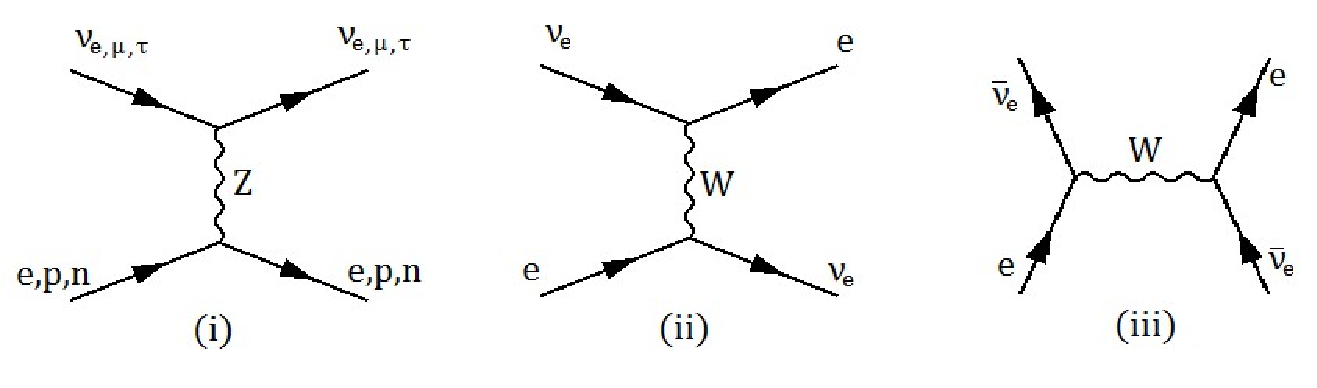
\includegraphics[width=0.9\textwidth]{figures/NC_and_CC_currents.pdf}
\centering
\caption{Neutrino interaction with matter. (i) All neutrinos participate in NC interactions which 
leads to additional effective mass for all eigenstates $\nu_1, \nu_2$ and $\nu_3$, (ii) Additional 
CC interaction for electron neutrino $\nu_e$, which modifies mass square difference, (iii) effect 
similar to (ii) only for electron anti-neutrino $\bar{\nu}_e$. The diagram (iii) contributes with 
opposite sign in comparison to (ii).} \lb{fig:NC}
\end{figure}

Each neutrino studied by the NOvA experiment travels more than 810 km through the Earth's crust.
While propagating through the earth, neutrinos interact with matterm, and these interactions
distort the neutrino oscillations. Since interaction going through 
exchange of only weak gauge bosons there are two types of possible interaction: (i) neutrino 
emits $Z$ boson - neutral current (NC) interaction and (ii) neutrino emits $W^\pm$ boson - 
charged current (CC) interaction. In matter, all three flavors of neutrinos interact through 
the exchange of $Z$ boson with electrons, protons and neutrons. For electron neutrino there 
is another possibility - interaction through exchange $W^+$ boson with electrons, as illustrated  
in figure \ref{fig:NC}.

Accounting for interactions between neutrinos and the Earth adds two additional 
terms to the Hamiltonian which describes neutrino propagation - an effective potential,
\be
V_{C} = \sqrt{2}G_{F}N_e \qquad and \qquad V_{N} = -\frac{1}{\sqrt{2}}G_{F}N_n,
\ee
where $G_F$ is Fermi constant, $N_e$ and $N_n$ electron and neutron number density respectively. 
The second term effectively shifts all $m_i^2 \rightarrow m_i^2 + 2|\mathbf{p}|V_N$ and does not 
have an effect on $\Delta m_{ij}$. The first term $V_C$ enters the Hamiltonian in a such way 
that it only affects the electron neutrino $\nu_e$ and electron anti-neutrino $\bar{\nu}_e$. After 
further calculations one derives the following 
corrected expressions for $\Delta m_{32}$ and $\sin 2\theta_{13}$ in the presence of matter
\be
\Delta m_{32}^2\Big|_{mat} = \sqrt{(\Delta m_{32}^2 \sin2\theta_{13})^2 + (\Delta m_{32}^2\cos2\theta_{13} \mp 2E_\nu V_C)^2} \nn
\ee
\be
\sin 2\theta_{13}\Big|_{mat} = \frac{\Delta m_{32}^2 \sin 2\theta_{13}}{\sqrt{(\Delta m_{32}^2 \sin2\theta_{13})^2 + (\Delta m_{32}^2\cos2\theta_{13} \mp 2E_\nu V_C)^2}}
\ee
The matter effect has a significant influence on the $\nu_e$ appearance probability, and in the first approximation
\be
P_{\nu_\mu \rightarrow \nu_e}(E,L)\Big|_{mat} = \Big(1 \pm \frac{2E_\nu V_C}{\Delta m_{32}^2}\Big)P_{\nu_\mu \rightarrow \nu_e}(E,L),
\ee
where the "+" sign is for the neutrino and the "-" sign is for the antineutrino. This effect 
is known as the Mikheyev-Smirnov-Wolfenstein (MSW) effect, and for the NOvA experiment it 
plays an important role in measuring the CP violating phase $\delta_{CP}$.
\begin{figure}
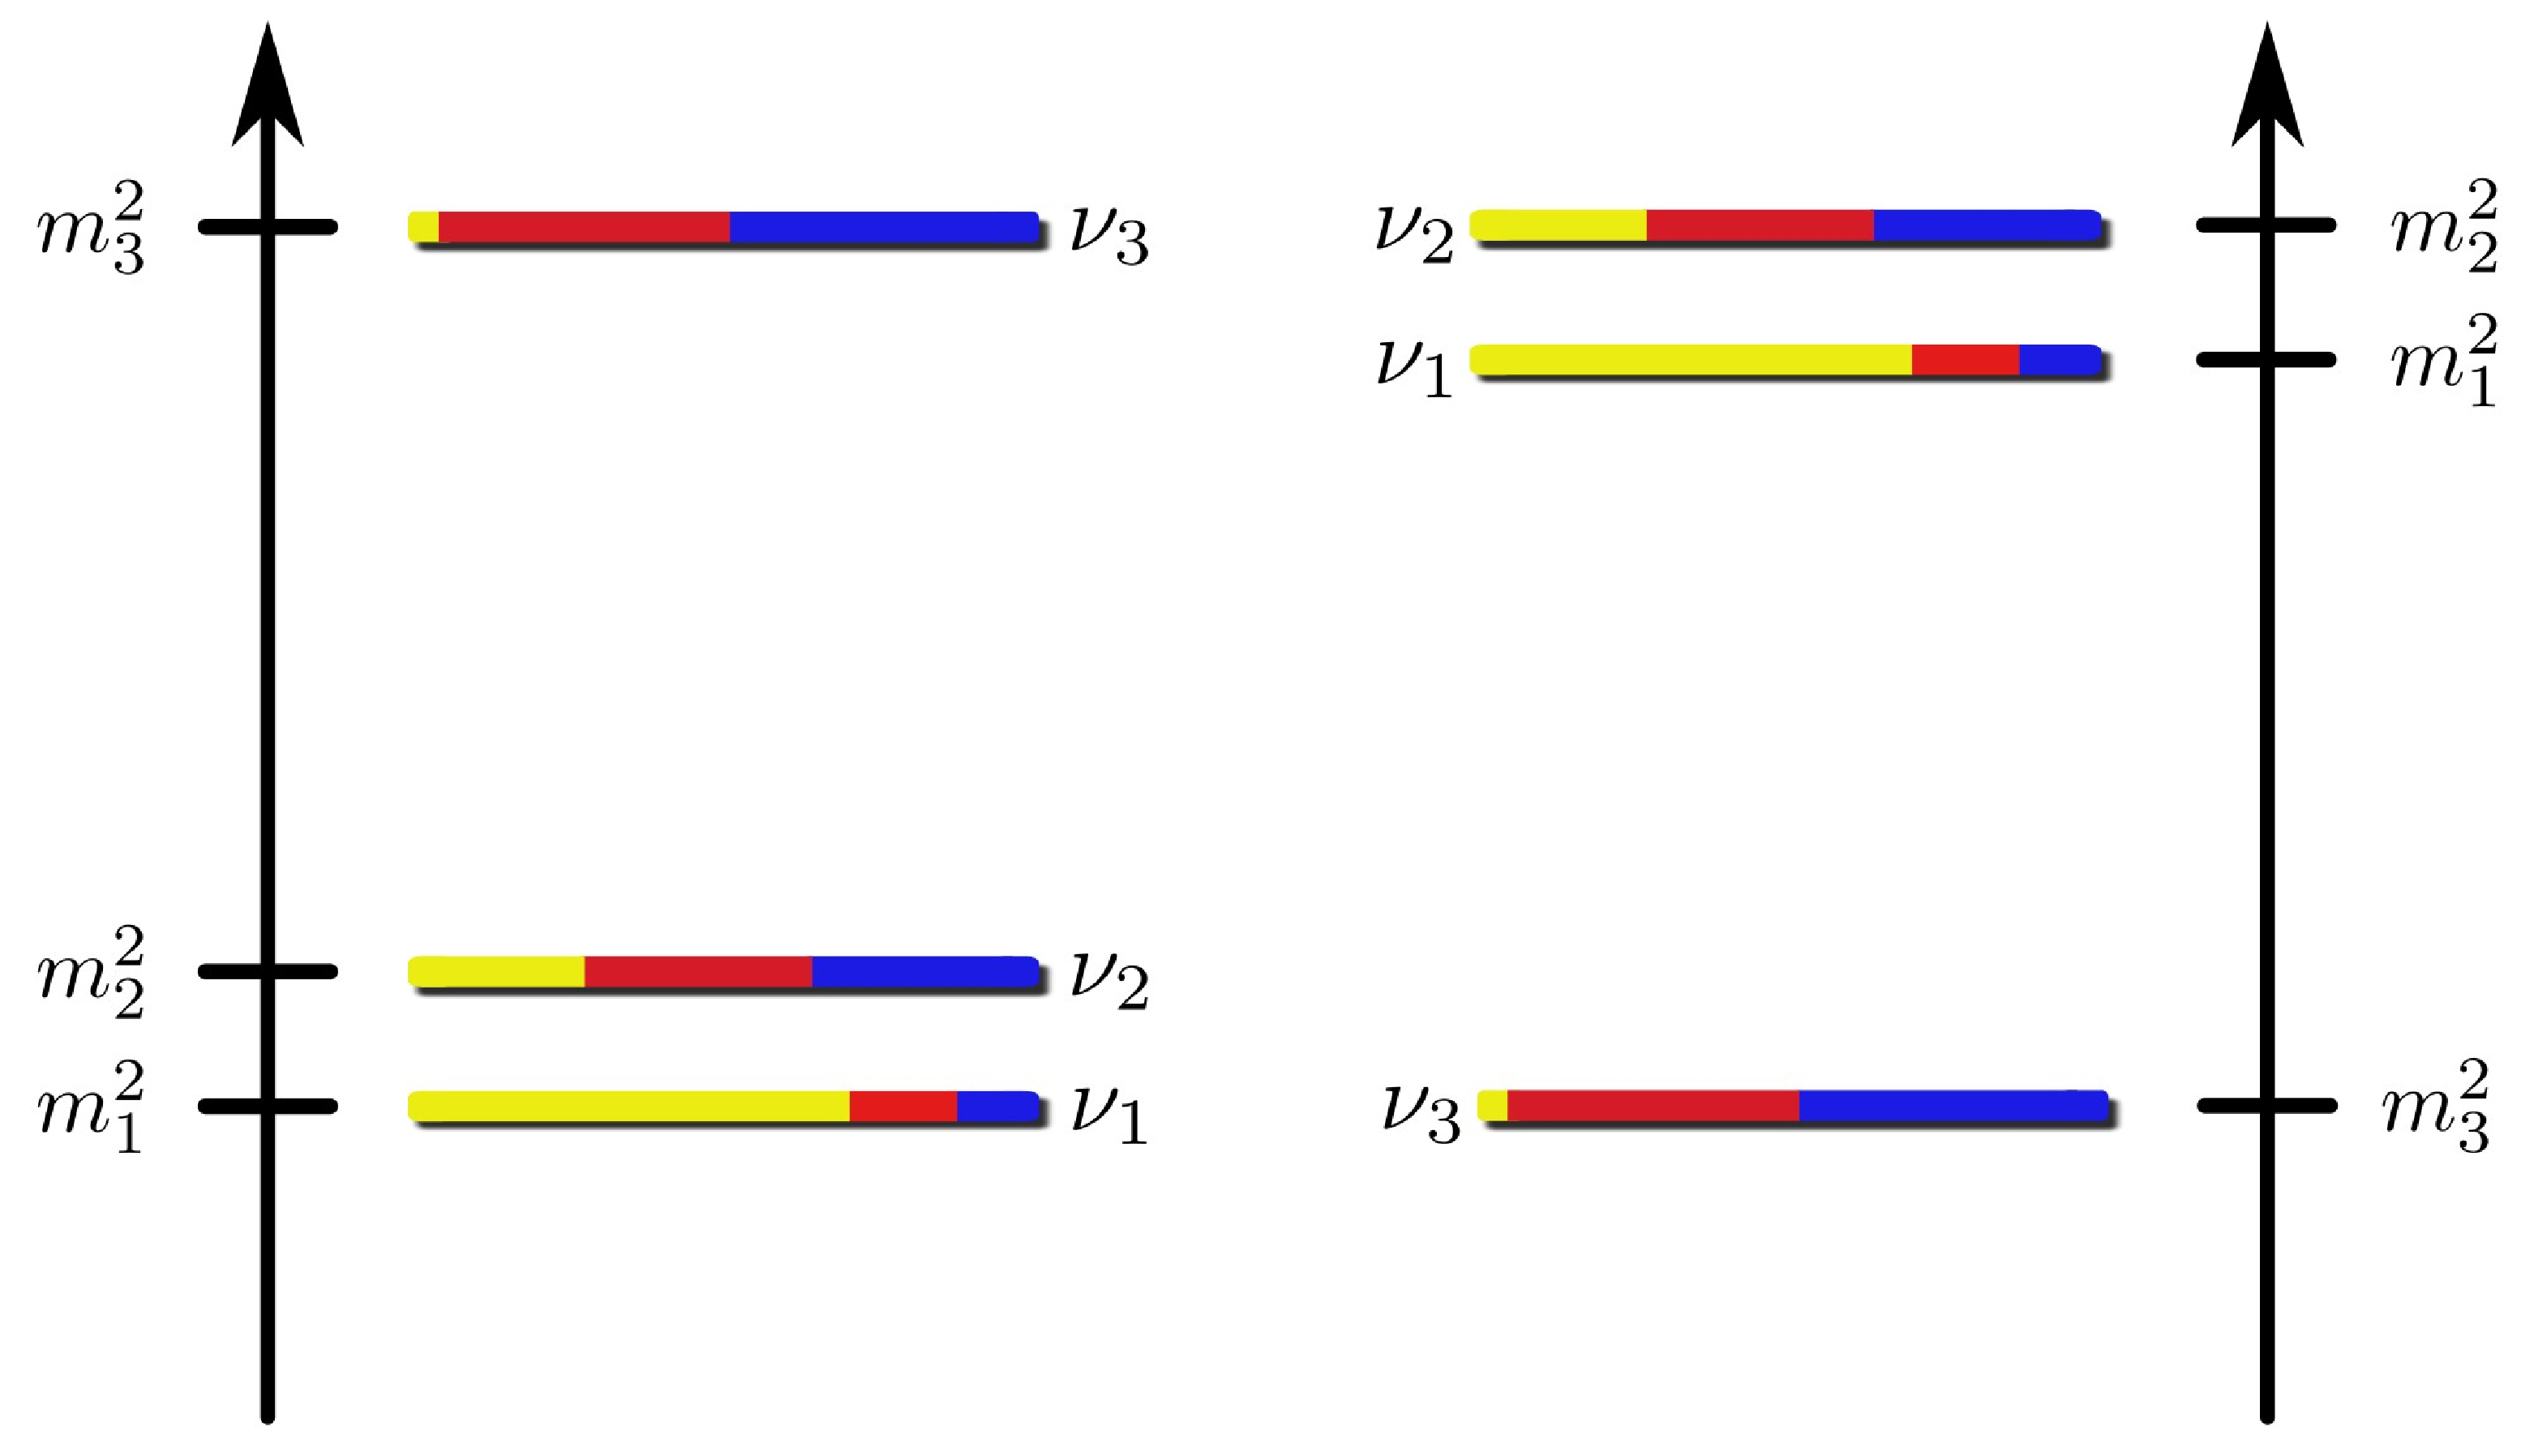
\includegraphics[width=0.9\textwidth]{figures/Nu_hierarchy.pdf}
\centering
\caption{Two possible variants of neutrino mass hierarchies. The left side corresponds to the normal 
hierarchy (NH) and right side corresponds to the inverted hierarchy (IH). Colors represent how much and 
what kind of neutrino flavors contribute to every mass state. The electron flavor is yellow, muon flavor 
is red and the tau flavor is blue.} \label{fig:NH}
\end{figure}

It is worth noting that assigning specific masses to specific mass states are completely 
arbitrary, but it is known from experimental data that two masses are much closer to each other 
in comparison with the third mass. These two masses are called $m_1$ and $m_2$, with $m_2 > m_1$ 
and $\Delta m_{12} << |\Delta m_{32}| \approx |\Delta m_{31}|$. However, the sign of $\Delta m_{32}$ 
is still unknown. That leaves two possibilities, called the normal hierarchy (NH) and the inverted 
hierarchy (IH). Figure \ref{fig:NH} illustrates the neutrino mass distributions. The NOvA experiment 
will be able to determine which hierarchy is realized in nature.

\section{Mixing Parameters Values} \label{osc_param}
Parameters which enter neutrino oscillation picture have to be detemined experimentally. Table \ref{cur_val}
shows the most recent, best fit measurements obtained in numerous experements. Two mass diferences are 
mesured and the measurements are making Figure \ref{fig:NH} to be not to scale. All three mixing angles
are also measured; it turns out that the third mass state almost does not have a contribution of electron 
flavor ($\theta_{13}$ is relatively small) and has almost equal contribution from muon and tau flavors
($\theta_{23}$ is close to $\frac{\pi}{4}$). From a theoretical point of view, the latter fact is very 
intriguing because the exact equality of $\theta_{23}$ and $\frac{\pi}{4}$ could reveal some hidden symmetries 
in the lepton sector of the Standard Theory. Measurements of $\delta_{CP}$ comes with a big uncertainty, 
however the uncertainty gets smaller as more data is gathered.
\begin{table}
\begin{center}
  \renewcommand{\arraystretch}{1.4}
  \begin{tabular}{| c | c |}
    \hline
    \textbf{Parameter}                & \textbf{Best Fit Value} \\ \hline \hline
    $\Delta  m_{21}^2,  10^{-5} eV^2$ & $7.53\pm 0.18$  \\ \hline
    $|\Delta m_{32}^2|, 10^{-3} eV^2$ & $2.45\pm 0.05~~(2.52\pm 0.05)$ \\ \hline
    $\sin^2(\theta_{12})$             & $0.307^{+0.013}_{-0.012}$ \\ \hline
    $\sin^2(\theta_{23})$             & $0.51\pm 0.04~~ (0.50\pm 0.04)$ \\ \hline
    $\sin^2(\theta_{13})$             & $0.0210\pm 0.0011$ \\ \hline
    $\delta_{CP}/\pi$                 & $0.0-2.0~~(0.0-0.1,~ 0.5-2.0)$  \\
    \hline
  \end{tabular}
\caption{Best fit values for the mixing parameters from latest edition of the Particle Data Group. Values in parenthesis are stated for the assumption of the inversed mass hierarchy, when no values in parenthesis are given that mean their are free of mass hierarchy assumption. The best fit values are given with 90\% CL.} \lb{cur_val}
\end{center}
\end{table}

The primary goal of NOvA is to measure $\theta_{13}$ and determine mass hierarchy, but it is also sensetive to $\theta_{23}$,
$m_{32}^2$, and $\delta_{CP}$. If nature prefers non-maximal mixing i.e., $\theta_{12} 
\neq \frac{\pi}{4}$, NOvA would be able to determine octant\footnote{Upper octant if $\theta_{23} > \frac{\pi}{4}$
and lower octant if $\theta_{23} < \frac{\pi}{4}$.}. In the current analysis, $\theta_{23}$ and 
$m_{32}^2$ are measured. 
%%%%%%%%%%%%%%%%%%%%%%%%%%%%%%%%%%%%%%%%%%%%%%%%%%%%%%%%%%%%%%%%%%%%%%%%%%%%%%%%

%%%%%%%%%%%%%%%%%%%%%%%%%%%%%%%%%%%%%%%%%%%%%%%%%%%%%%%%%%%%%%%%%%%%%%%%%%%%%%%%
